
\documentclass[a4paper,12pt]{article}
\usepackage[a4paper,top=1.3cm,bottom=2cm,left=1.5cm,right=1.5cm,marginparwidth=0.75cm]{geometry}
\usepackage{cmap}					
\usepackage[warn]{mathtext} 		
\usepackage[T2A]{fontenc}			
\usepackage[utf8]{inputenc}			 
\usepackage[english,russian]{babel}	
\usepackage{longtable}
\usepackage{float}
\restylefloat{table}
\usepackage{graphicx}
\usepackage{tabularx}
\usepackage{hyperref}
\usepackage[rgb]{xcolor}
\usepackage{amsmath,amsfonts,amssymb,amsthm,mathtools} 
\mathtoolsset{showonlyrefs=true}
\usepackage{euscript}
\usepackage{mathrsfs}
\date{\today}
\begin{document}

\begin{titlepage}
	\begin{center}
		{\large МФТИ}
	\end{center}
	\begin{center}
		{\large ФРКТ}
	\end{center}
	
	
	\vspace{4.5cm}
	{\huge
		\begin{center}
			{\bf Отчёт о выполнении лабораторной работы 4.5.2}\\
		  Интерференция лазерного излучения.
		

		\end{center}
	}
	\vspace{9cm}
	\begin{flushright}
		{\LARGE  Добровольская Ксения 
			\vspace{0.2cm}
			Б01-101}\\
		{\LARGE  Гаврилин Илья 
			\vspace{0.2cm}
			Б01-101}
	\end{flushright}
	\vspace{8cm}
	
\end{titlepage}

\section{Аннотация}

  В данной лабораторной работе мы исследовали видность интерференционной картины излучения гелий-неонового лазера и определили длину когерентности излучения. Также мы исследовали поляризацию используемного в установке лазера, сравнивая теоретические зависимости с экспериментальными, получили линейную поляризацию.
  
  
  В работе использовались: гелий-неоновый лазер, интерферометр Майкельсона с подвижным зеркалом, фотодиод с усилителем, осциллограф, поляроид, линейка.
  
\section{Измерение видности.} 

  \begin{figure}[H]
  \begin{center}
    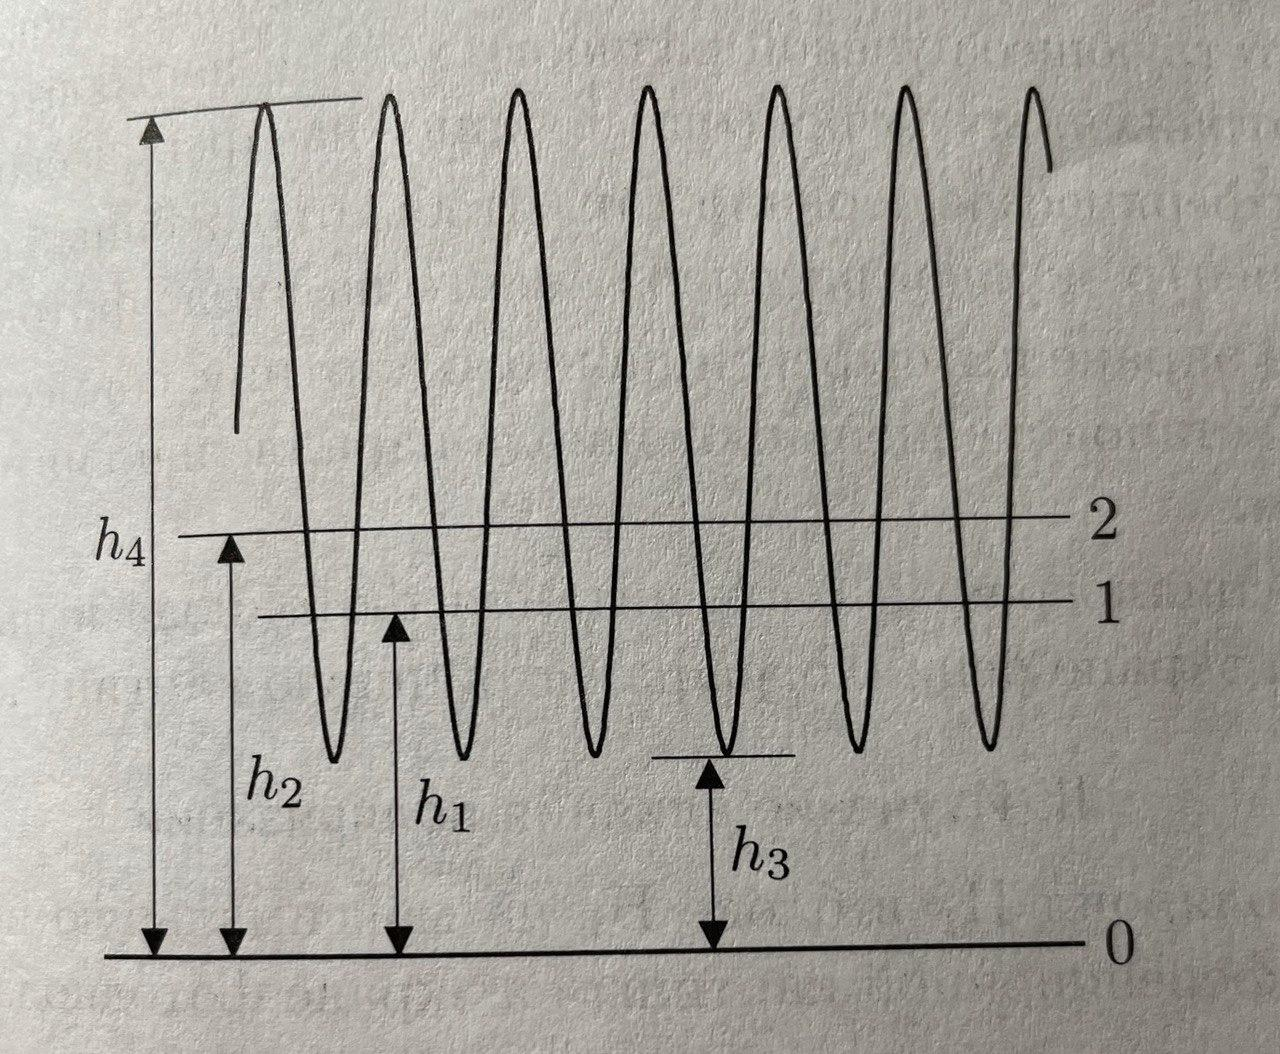
\includegraphics[width=9 cm]{ex2.jpg}
    \caption{Осциллограмма сигналов с фотодиода.}
    \label{fig:}
  \end{center}
\end{figure}

 В работе требуется измерять видность следующим способом.
 
 При перемещении поперек интерференционной картины разность фаз изменяется, и мы переходим от одного максимума к другому. При этом интенсивность в максимуме $Imax = (Am + Bm)^2$ , а в минумуме $Imin = (Am - Bm)^2$. Поэтому видность 
 
\[ \nu_1 = \frac{2\sqrt{\delta }}{1 + \delta} \],

где введен параметр $\delta  = \frac{(B_m)^2 }{A_m)^2}$. 

На рис.2. можно найти следующие величины 


0 - фоновая засветка (во всех измерениях принимает значение 1)


1 - перекрыт пучок 2


2 - перекрыт пучок 1


3,4 - открыты оба пучка


При этом параметр  $\delta =\frac{h_1}{h_2}$.


Видность интерференционной картины рассчитывается по формуле


\[\nu = \frac{h_4 - h_3}{h_4 + h_3} \].


Затем можно определить видность при данной разности хода l для угла между плоскостями поляризации пучков $\beta = 0 (\nu_3 = 1)$.

\[ \nu_2(l) = \frac{\nu }{\nu_1} \]


или при l = 0, ($\nu_2 = 1)$ для известного угла $\beta$:


\[ \nu_3(\beta ) = \frac{\nu }{\nu_1} \]
 
  
\section{Экспериментальная установка.} 

  Для получения интерференционной картины используется интерферометр Майкельсона, смонтированный на вертикально стоящей массивной металлической плите. Схема установки приведена на рас.1.
  
    
  \begin{figure}[H]
  \begin{center}
    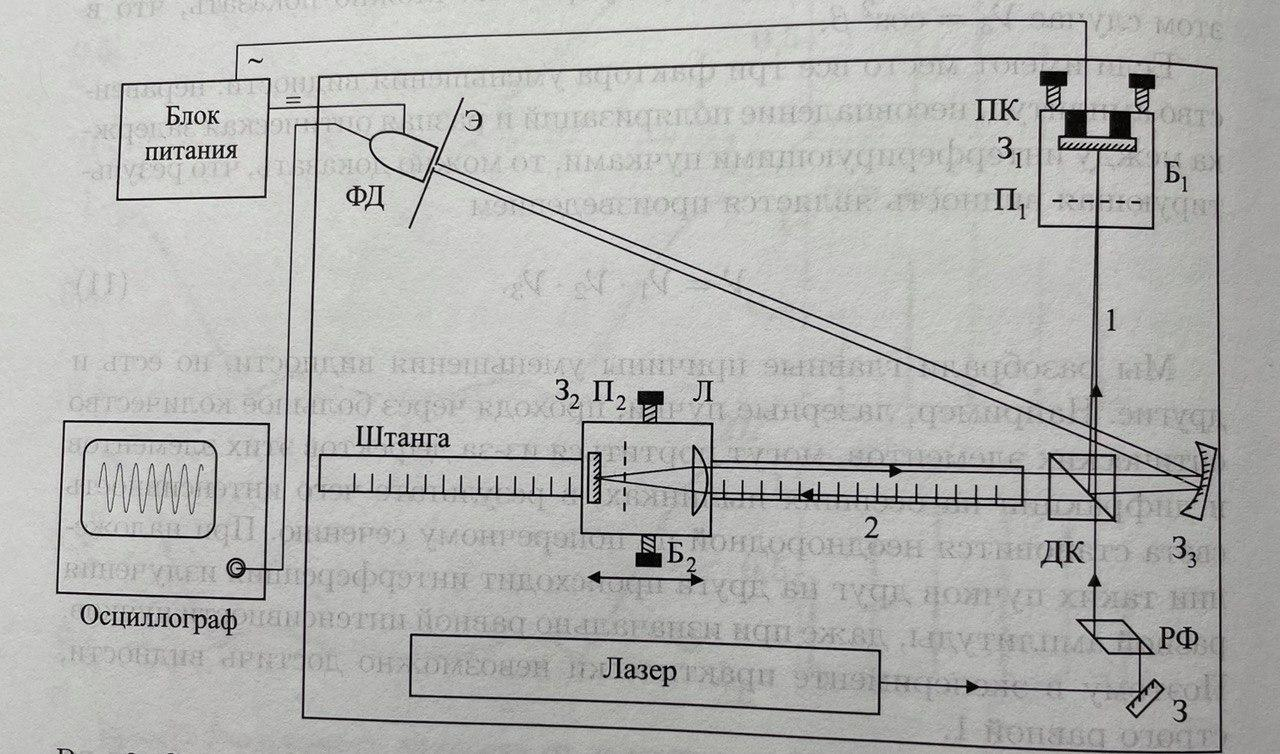
\includegraphics[width=15cm]{ex1.jpg}
    \caption{Схема экспериментальной установки}
    \label{fig:}
  \end{center}
\end{figure}

  Пучок гелий-неонового лазерного излучения со средней длиной волны 633 нм отражается от зеркала З и проходит призму полного внутреннего отражения РФ(ромб Френеля), которая превращает линейную поляризацию излучения в круговую. Далее излучение кубиком ДГ делится на два луча, один из которых проходит черер поляроид и отражаясь от зеркала З3 попадает на фотодиод, а другой проходит через линзу и поляроид П2 и отразившись от зеркаа З2 и затем зеркала З3 также попадает на фотодиод ФД. 
  
  Таким образом, на фотодиод приходят два пучка, прошедшие разные плечи интерферометра. Они интерферируют и создают интерференционные полосы. Сферическое зеркало З3 с небольшим фокусным расстоянием увеличивает картину интерференционных полос и позволяет наблюдать ее на экране Э.
  
  


\section{Измерение видности в зависимости от угла $\beta  $.} 

В работе мы измеряем зависимость видности интерференционной картины от угла между плоскостями поляризации интерферирующих волн при нулевой разности хода. По результатам измерений оцениваем спектральные характеристики лазерного излучения: .

\begin{enumerate}

\item Поворачиваем поляроид и с помощью шкалы измеряем угол поворота $\beta (\nu_2 = 1).$ 
\item Измеряем величины $h_1, h_2, h_3, h_4$ на экране осциллографа:



\begin{table}[H]
\begin{center}
\begin{tabular}{|c|c|c|c|c|c|c|c|c|c|c|}
\hline $\beta  $&180&170&160&150&140&130&120&110&100&90\\
\hline $h_1$&4.0&4.5&4.2&4.5&4.4&4.5&4.5&4.5&4.5&4.5\\
\hline $h_2$&5.5&5.0&5.8&3.9&2.5&2.0&2.0&1.5&1.2&1.1\\
\hline $h_3$&2.0&2.0&2.1&2.0&2.5&3.0&3.1&3.9&4.0&5.0\\
\hline $h_4$&16.0&15.0&16.9&13.0&9.5&8.1&8.0&5.5&5.7&5.0\\
\hline $\nu $&0.78&0.76&0.74&0.73&0.58&0.46&0.44&0.17&0.16&0\\
\hline $\delta$&0.73&0.9&0.72&1.15&1.76&2.3&2.3&3.0&3.8&4.1\\
\hline $\nu_3$&0.79&0.76&0.75&0.73&0.60&0.50&0.48&0.20&0.18&0\\
\hline 
\end{tabular}
\end{center}
\end{table}


  Строим график $\nu_3(\beta)$.


\begin{figure}[H]
  \begin{center}
    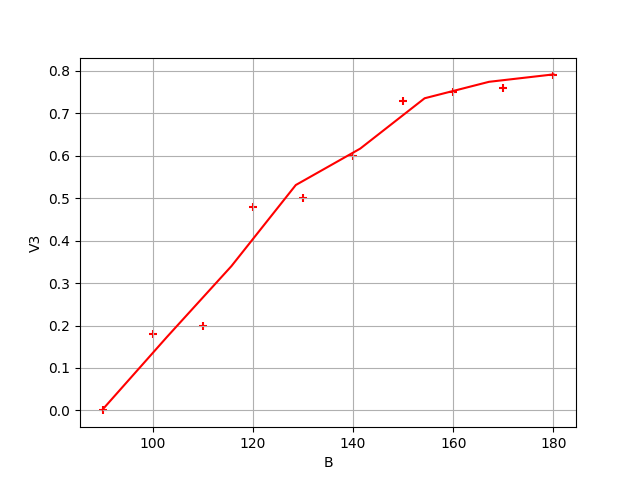
\includegraphics[width=13cm]{gra1.png}
    \caption{График зависимости видности интерференционной картины от угла между плоскостями поляризации интерферирующих волн при нулевой разности хода.}
    \label{fig:}
  \end{center}
\end{figure}

\item Сравнивая полученные значения с теоретическими зависимостями $\nu_3 = cos\beta , \nu_3 = (cos\beta )^2$ можем видеть, что первая ближе к измеренным данным, значит на основании этого наблюдения можно сказать о линейной поляризации излучения используемного в установке лазера.
  
  \begin{figure}[H]
  \begin{center}
    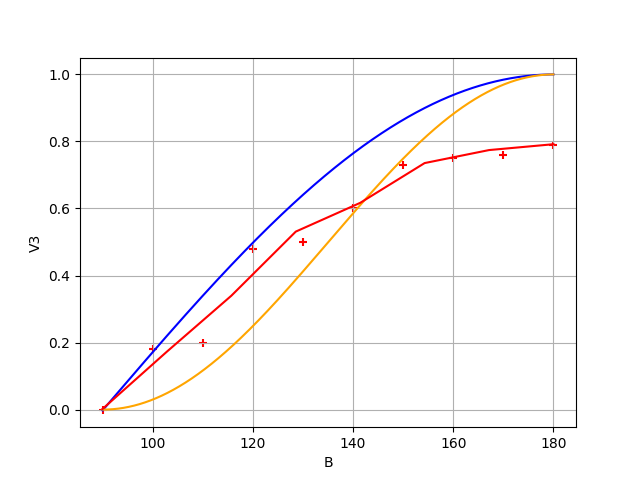
\includegraphics[width=13cm]{gra2.png}
    \caption{Сравнение экспериментальной зависимости с теоретическими.}
    \label{fig:}
  \end{center}
\end{figure}

\end{enumerate}


\section{Измерение видности в зависимости от положения каретки  $x$.} 
Теперь установим $ \alpha $ на максимальную видность и будем перемещать блок $ Б_2 $, тем самым изменяя дальность хода $ x $. Аналогично предыдущему пункту измерим величины $ h_1, h_2, h_3 \; и \; h_4 $ на экране осциллографа. Результаты занесем в таблицу и построим график согласно формуле для $V_2$. Значения для $ \delta, V, V_1 $ получим из формул выше.

\begin{table}[H]
	\centering
	\begin{tabular}{|c|c|c|c|c|c|c|c|c|}
		\hline
		$x$, см  & $h_1$, см & $h_2$, см & $h_3$, см & $h_4$, см & V     & $\delta$ & $V_1$  & $V_2$  \\ \hline
		16 & 4    & 11   & 5    & 23   & 0.643 & 0.364 & 0.884 & 0.727 \\ \hline
		18 & 7.5  & 2.8  & 3.8  & 15   & 0.596 & 2.679 & 0.890 & 0.670 \\ \hline
		20 & 1.1  & 6.8  & 5    & 9    & 0.286 & 0.162 & 0.692 & 0.413 \\ \hline
		22 & 2.2  & 6.2  & 4    & 11.5 & 0.484 & 0.355 & 0.879 & 0.550 \\ \hline
		24 & 6    & 4.4  & 4    & 12   & 0.500 & 1.364 & 0.988 & 0.506 \\ \hline
		26 & 5    & 9    & 8    & 13   & 0.238 & 0.556 & 0.958 & 0.248 \\ \hline
		28 & 2    & 7    & 5.5  & 10   & 0.290 & 0.286 & 0.831 & 0.349 \\ \hline
		30 & 10   & 5    & 10   & 16   & 0.231 & 2.000 & 0.943 & 0.245 \\ \hline
		32 & 8    & 6    & 11   & 15   & 0.154 & 1.333 & 0.990 & 0.155 \\ \hline
		42 & 6.3  & 6.8  & 11   & 13   & 0.083 & 0.926 & 0.999 & 0.083 \\ \hline
		44 & 1.8  & 5.2  & 5.5  & 6.5  & 0.083 & 0.346 & 0.874 & 0.095 \\ \hline
		54 & 5    & 1    & 5.8  & 6.2  & 0.033 & 5.000 & 0.745 & 0.045 \\ \hline
		56 & 4.8  & 1    & 5.5  & 6    & 0.043 & 4.800 & 0.755 & 0.058 \\ \hline
		58 & 5.5  & 1    & 6.2  & 6.4  & 0.016 & 5.500 & 0.722 & 0.022 \\ \hline
		60 & 4.5  & 2.4  & 6.5  & 7.4  & 0.065 & 1.875 & 0.953 & 0.068 \\ \hline
		62 & 2.8  & 2.3  & 4.2  & 5.6  & 0.143 & 1.217 & 0.995 & 0.144 \\ \hline
		64 & 1    & 2    & 2.8  & 4    & 0.176 & 0.500 & 0.943 & 0.187 \\ \hline
		66 & 4    & 2    & 4.3  & 8    & 0.301 & 2.000 & 0.943 & 0.319 \\ \hline
		68 & 0.5  & 2    & 1.8  & 4.8  & 0.455 & 0.250 & 0.800 & 0.568 \\ \hline
		70 & 2.5  & 2    & 3    & 7.6  & 0.434 & 1.250 & 0.994 & 0.437 \\ \hline
		72 & 2.8  & 2    & 2.4  & 7.2  & 0.500 & 1.400 & 0.986 & 0.507 \\ \hline
		74 & 2.2  & 1.3  & 1.8  & 5.5  & 0.507 & 1.692 & 0.966 & 0.524 \\ \hline
		76 & 2.2  & 2.5  & 2    & 7.2  & 0.565 & 0.880 & 0.998 & 0.566 \\ \hline
		78 & 1.8  & 2.8  & 2.4  & 6.6  & 0.467 & 0.643 & 0.976 & 0.478 \\ \hline
		80 & 1.2  & 2.8  & 2.3  & 5.3  & 0.395 & 0.429 & 0.917 & 0.431 \\ \hline
	\end{tabular}
	\caption{ Видность в зависимости от положения каретки  $x$}
\end{table}
\begin{figure}[H]
	\centering
	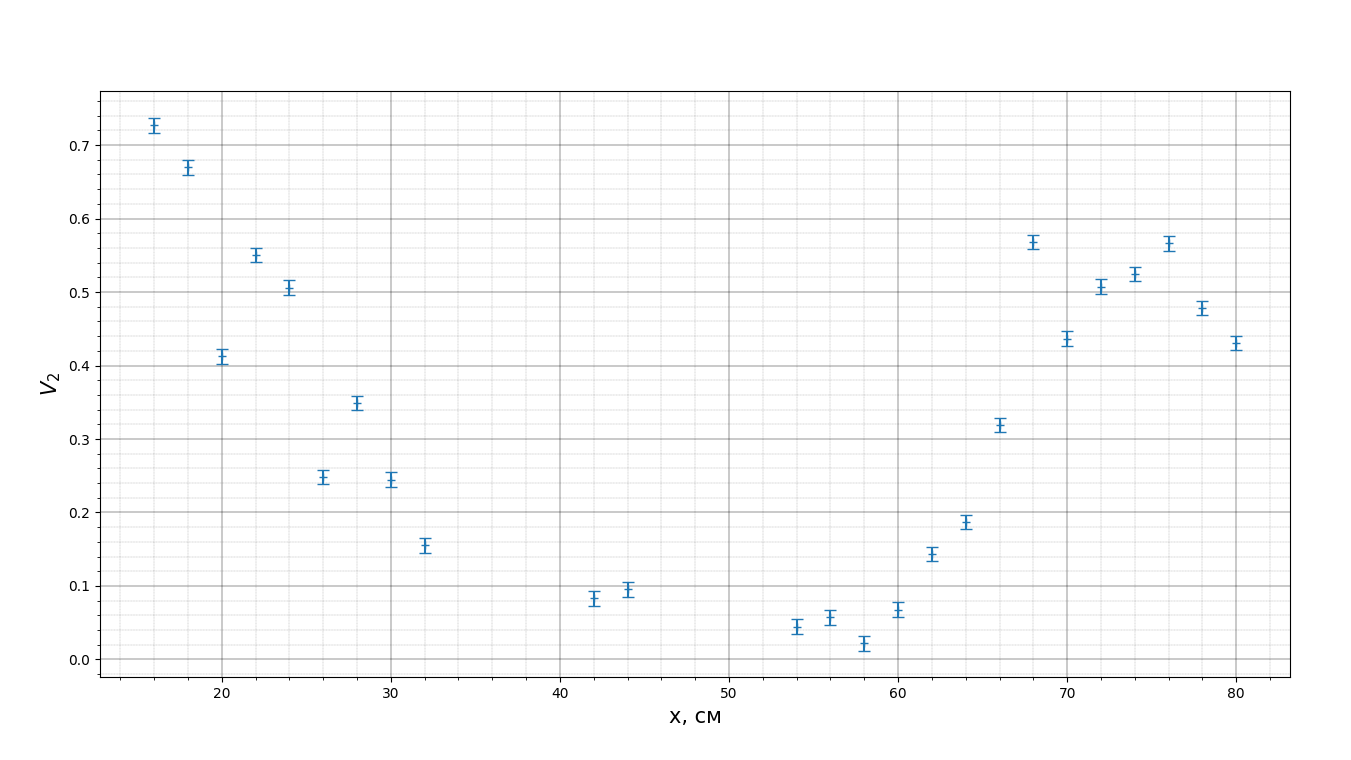
\includegraphics[width=0.8\linewidth]{Figure_1}
	\caption{Видность в зависимости от положения каретки  $x$}
	\label{fig:figure1}
\end{figure}

Видно, что у нас наблюдается 2 максимума по краям области измерения и некоторые колебания в промежуточной области. А именно, максимумы в области $ x_1 \approx (10 \pm 2) \; см $ и в области $ x_2 \approx (75 \pm 2) \; см $, откуда получаем следующий результат:

\begin{equation}\label{}
	L = \dfrac{1}{2} (x_2 - x_1) = (32,5 \pm 1,4) \; см
\end{equation}

Отсюда нетрудно получить и значение $ \Delta \nu $:

\begin{equation}\label{}
	\Delta \nu = \frac{c}{2L} \approx (4,6 \pm 0,2) \cdot 10^8 \; Гц
\end{equation}

Оценим $ l_{1/2} \approx 18 - 10 = 8 \pm 2 $
\begin{equation}\label{}
	2 \Delta F = 2 \cdot \frac{0,26 c}{l_{1/2}} \approx (19,5 \pm 4,9) \cdot  10^8 Гц
\end{equation}

Тогда для числа одновременно генерируемых лазером продольных волн можно провести оценку:

\begin{equation}\label{}
	N \approx 1 + \dfrac{ 2\Delta F}{\Delta \nu} \approx 5 \pm 1
\end{equation}




\section{Обсуждение результатов и выводы}

В данной лабораторной работе мы: 


1. Исследовали зависимость видности интерференционной картины излучения гелий-неонового лазера от угла между плоскостями поляризации интерферирующих волн при нулевой разности хода. Сравнивая теоретические зависимости с экспериментальными, получили линейную поляризацию.

2. Исследовали зависимость видности интерференционной картины излучения гелий-неонового лазера от разности хода интерферирующих пучков для нулевого угла между плоскостями поляризации.

3. По результатам измерений оценили спектральные характеристики лазерного излучения: ширину спектра генерации и число генерируемых мод.

$\newline$




\end{document}
	
